\documentclass[11pt]{article}
\usepackage{natbib}
\usepackage{float}
\usepackage[textwidth=6.5in,textheight=8.5in]{geometry}
\usepackage{changepage}
\usepackage[pdftex]{graphicx}     % could insert ``draft'' between []
\usepackage{amsmath}
\usepackage{amssymb}
\pagestyle{empty}
\setlength{\oddsidemargin}{0pt}
%\setlength{\textwidth}{6.5in}
\setlength{\voffset}{0pt}
\setlength{\topmargin}{-0.25in}
%\setlength{\textheight}{8.5in}
\extrafloats{120}
%%%%%%%%%%%
\newcommand\aj{AJ}%
          % Astronomical Journal
\newcommand\actaa{\ref@jnl{Acta Astron.}}%
  % Acta Astronomica
\newcommand\araa{\ref@jnl{ARA\&A}}%
          % Annual Review of Astron and Astrophys
\newcommand\apj{ApJ}%
          % Astrophysical Journal
\newcommand\apjl{\ref@jnl{ApJ}}%
          % Astrophysical Journal, Letters
\newcommand\apjs{\ref@jnl{ApJS}}%
          % Astrophysical Journal, Supplement
\newcommand\ao{\ref@jnl{Appl.~Opt.}}%
          % Applied Optics
\newcommand\apss{\ref@jnl{Ap\&SS}}%
          % Astrophysics and Space Science
\newcommand\aap{\ref@jnl{A\&A}}%
          % Astronomy and Astrophysics
\newcommand\aapr{\ref@jnl{A\&A~Rev.}}%
          % Astronomy and Astrophysics Reviews
\newcommand\aaps{\ref@jnl{A\&AS}}%
          % Astronomy and Astrophysics, Supplement
\newcommand\icarus{\ref@jnl{Icarus}}%
  % Icarus
\newcommand\mnras{\ref@jnl{MNRAS}}%
          % Monthly Notices of the RAS
\newcommand\prc{\ref@jnl{Phys.~Rev.~C}}%
          % Physical Review C
\newcommand\prd{\ref@jnl{Phys.~Rev.~D}}%
          % Physical Review D
\newcommand\pre{\ref@jnl{Phys.~Rev.~E}}%
          % Physical Review E
\newcommand\prl{\ref@jnl{Phys.~Rev.~Lett.}}%
          % Physical Review Letters
\newcommand\pasa{\ref@jnl{PASA}}%
  % Publications of the Astron. Soc. of Australia
\newcommand\pasp{\ref@jnl{PASP}}%
          % Publications of the ASP

\newcommand{\kvec}{{\bf k}}
\newcommand{\bvec}{{\bf b}}
\newcommand{\shat}{{\hat s}}
\newcommand{\kpr}{{k_\perp}}
\newcommand{\kvpr}{{\kvec_\perp}}
\newcommand{\kpl}{{k_\parallel}}
\newcommand{\AI}{{\langle\tilde A*\tilde I\rangle}}
\newcommand{\AItau}{{\AI(\tau)}}
\newcommand{\hMpci}{{h~{\rm Mpc}^{-1}}}
\newcommand{\inch}{$^{\prime\prime}$}
\newcommand{\foot}{$^{\prime}$}
\renewcommand{\deg}{^\circ}
\newcommand{\integral}{\int\limits}


\begin{document}
\title{Some HERA System Definitions: I}
\author{David DeBoer, Eloy de Lera Acedo}
\maketitle

\begin{center}
{\bf Abstract}
\end{center}

\small
\begin{adjustwidth}{1in}{1in}
This note defines some system characterization parameters in the context of HERA observations.  It mostly adheres to IEEE definitions.  The defined parameters are in bold and are: antenna normalized power pattern, directive gain, gain pattern, gain, antenna efficiency, effective area, aperture efficiency, beam solid angle, antenna temperature, receiver temperature, system temperature, sensitivity and SEFD.
\end{adjustwidth}

\section{Antenna Properties}
The {\bf Antenna Normalized Power Pattern}, $P(\theta,\phi)$, is described by the ratio of the power received from a point source at infinity as a function of pointing direction to its maximum value.  We define this maximum pointing direction to occur at $\theta = \phi = 0$ and call it ``boresight''.  If we measure power in arbitrary units as a function of pointing as $W(\theta,\phi)$, then
\begin{equation}
P(\theta,\phi) = \frac{W(\theta,\phi)}{W(0,0)}
\end{equation}
This is unitless and usually plotted in decibels as $P$[dB] = 10log$_{10}(P)$.

The {\bf Directive Gain} of an antenna, $D(\theta,\phi)$, is another ``pattern'' but normalized to the power received by a (theoretically impossible) isotropic antenna.  It may be expressed as:
\begin{equation}
D(\theta,\phi) = \frac{4\pi P(\theta,\phi)}{\int\int P(\theta,\phi)d\Omega}
\end{equation} 
This is also dimensionless, but is also usually plotted as ''decibels relative to isotropic'' $D$[dBi] = 10log$_{10}(D)$.

The {\bf Directivity} of an antenna, $D$ without the $(\theta,\phi)$, is the directive gain value at its maximum value, which we've defined as boresight:  $D = D(0,0)$.

The {\bf Gain Pattern} of an antenna, $G(\theta,\phi)$, is the directive gain reduced by any other losses not caught in integrating the beam pattern.  This comes from things like ohmic losses and leakage, which we lump into an efficiency parameter we'll denote $\eta_R$
\begin{equation}
G(\theta,\phi) = \eta_R D(\theta,\phi)
\end{equation}
Since the input reference point has been specified at the antenna terminals, things like mismatch are ignored here.  They are present in the real system and must be included in the full system analysis.

The {\bf Gain} of an antenna, $G$ without the $(\theta,\phi)$, is the value of the gain pattern at boresight:  $G = \eta_R D$.

Note that typically $\eta_R \approx 1$, so that $D$ and $G$ are generally quite close to each other in value and we often and confusingly use them interchangeably, but if you care about the details don't forget about $\eta_R$ (and don't forget whether you mean at boresight, or at some other angle).

The {\bf Antenna Efficiency}, $\eta$, is the ratio of the  {\bf Effective Area} of an antenna, $A_e$, to the geometric area of the antenna, $A_g$ (this serves to circuitously define both $\eta$ and $A_e$).  So,
\begin{equation}
A_e = \eta A_g
\end{equation}
Note that we may define an {\bf Aperture Efficiency}, $\eta_A$, as
\begin{equation}
\eta_A = \frac{4\lambda^2}{\pi d^2\Omega_A}
\end{equation}
where $d$ is the diameter and $\Omega_A$ is the {\bf Beam Solid Angle} defined as
\begin{equation}
\Omega_A = \int \int P(\theta,\phi)d\Omega
\end{equation}
Then we find that $\eta = \eta_A \eta_R$.

Finally, we note that we can relate effective area to gain by
\begin{equation}
G = \eta_R D = \eta_R \eta_A\left(\frac{\pi d}{\lambda}\right)^2
\end{equation}
Note that this also means we could define the effective area as a function of pointing angle, however generally we mean it to be at boresight.  Also, a lot of ``efficiencies'' are absorbed in the terms above, which I've left out of scope here.

\section{Temperatures}
This will present a very simple set of temperature definitions appropriate for HERA observations.  For a perfect and noiseless system, the power present at the antenna terminals from the sky for a pointing direction ($\theta, \phi$) in bandwidth $\Delta\nu$ is
\begin{equation}
W(\theta,\phi) = \frac{1}{2}A_e\int \int B(\theta^\prime,\phi^\prime)P(\theta^\prime-\theta,\phi^\prime-\phi)d\Omega^\prime \Delta \nu
\end{equation}
where $B(\theta,\phi)$ is the sky brightness.  
Comparing this to the power from just a resistor at temperature $T$ ($w = kT\Delta\nu$) we can define an equivalent {\bf Antenna Temperature}, $T_A$ as
\begin{equation}
\label{Eq:TA}
T_A =  \frac{A_e}{2k}\int \int B(\theta^\prime,\phi^\prime)P(\theta^\prime-\theta,\phi^\prime-\phi)d\Omega^\prime
\end{equation}

Of course, we don't have a perfect, noiseless receiver (still working on it), so that it also injects noise into the system.  We define that extra noise as the {\bf Receiver Temperature}, $T_R$.  Note that even though it is injected throughout the receiver, we pretend it is all injected at the antenna terminals as well (we call that the ``input-referred noise temperature'').  If we make sure to do that, the total power available at the antenna terminals (expressed as temperature) is the {\bf System Temperature}, which has components from the sky, the antenna and the receiver.  It is given by
\begin{equation}
T_{sys}(\nu) = \eta_R T_A(\nu) + (1-\eta_R)T_p + T_R(\nu) \approx T_A(\nu) + T_R(\nu)
\end{equation}
where $T_p$ is the physical temperature.
Note that all of these quantities are functions of frequency, so I've added that dependency to remind us.

The power that we record goes through the vagaries of being received (so amplified and noisified).  The power we record over a bandwidth $\Delta\nu$ is then
\begin{equation}
P = kG_{sys}T_{sys}\Delta\nu
\end{equation}
however, we {\em always} specify noise temperatures as input-referred.  So, if someone says ``the receiver temperature is 100 K'' and you are looking at blank sky, 
the system temperature will be 
\begin{equation}
T_{sys} = 100 + T_{cmb} + T_{sp} + T_{atm} ~~~~~~K 
\end{equation}
where $T_{sky}$ is the integral for $T_A$ over the upper hemisphere, $T_{sp}$ is the ``spill-over'' temperature (integral over the lower hemisphere {\em not} looking at the sky) and $T_{atm}$ is the radiometric temperature of the atmosphere.  Note that $T_{sp}$ and $T_{atm}$ are contained in the $T_A$ part, however it is convenient to have them separate to spare the poor astronomer from having to keep track of our (currently) life-sustaining planet.  $T_{atm}$ is generally negligible (impacted by the ionosphere at our frequencies).  See Fig. \ref{Fig:Tspill} for the spillover temperature for HERA (using Nicolas' beam patterns but assuming half goes back onto the sky + an added 10 K guess for the missing middle) and PAPER (using my somewhat quickly calculated HFSS model).

\begin{figure}[ht]
\centering
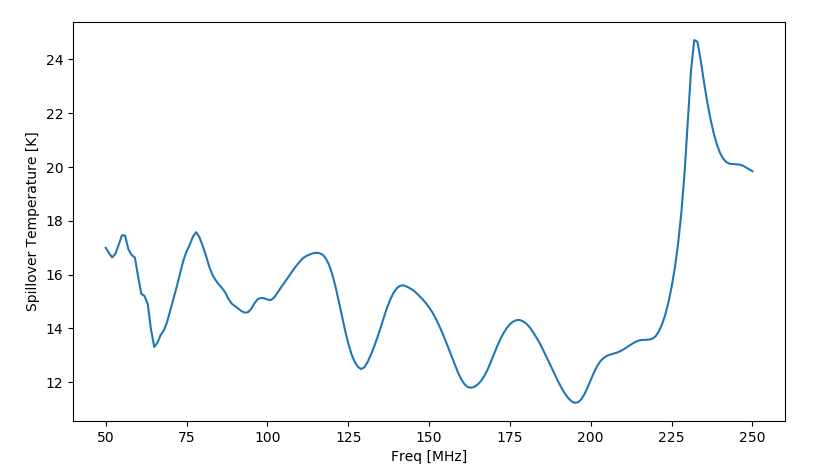
\includegraphics[width=0.65\textwidth]{spillover.png}
\caption{\small Estimate of the HERA and PAPER spillover temperatures.  Uses the Cavendish beams, but assumes half of that power goes back on the sky given all of the adjacent metal and adds in 10 K as an estimate of the contribution from the central hole.  This will go away if a central cone is used.  PAPER uses my quick HFSS-calculated beams.}
\label{Fig:Tspill}
\end{figure}

Note that if the source field is expressed in brightness temperature $T_B$, then
\begin{equation}
\label{Eq:TA}
T_A =  \frac{D}{4\pi}\int \int T_B(\theta^\prime,\phi^\prime)P(\theta^\prime-\theta,\phi^\prime-\phi)d\Omega^\prime
\end{equation}
where $D$ is the directivity.

\section{Sensitivity Parameters}
We define the {\bf Sensitivity} of an antenna, $\Gamma$, as
\begin{equation}
\Gamma = \frac{A_e}{2k}
\end{equation}
which we generally express in units of Kelvin per Jansky [K/Jy].  Therefore we can rewrite Eq. \ref{Eq:TA} as
\begin{equation}
T_A =  \Gamma \int \int B(\theta^\prime,\phi^\prime)P(\theta^\prime-\theta,\phi^\prime-\phi)d\Omega^\prime
\end{equation}

Another parameter used is the {\bf Source Equivalent Flux Density} ($SEFD$) which can be thought of in two different ways:
\begin{enumerate}
	\item it is the strength of a point source at boresight that would double the system temperature
	\item it is the system temperature expressed in Jansky
\end{enumerate}
They both equivalently yield
\begin{equation}
SEFD = \frac{T_{sys}}{\Gamma} = \frac{2kT_{sys}}{A_e}
\end{equation}

Note that the SEFD ({\em i.e.} the ratio $A_e/T_{sys}$) is the ``native'' measurement made by an antenna.  Separating the two quantities requires additional information and is generally difficult to do very accurately. 

\section{Polarization}
Polarization complicates things.  For antenna work, we generally work in relative polarization and we measure/compute co-polar and cross-polar beam patterns.  These are either orthogonal linear (which we are denoting E and N) or circular polarizations (RH/LH).
Although it is not how it is actually done, it is instructive to think of the antenna under test as fixed to looking at zenith and we run another transmitter antenna around on a great circle and measure what we get.

For co-polar, 

What else?

\section{Matching}
The impedance matching between the antenna and the first stage LNA has a dominant effect in the passband response of the system. It both affects the passband gain of the LNA and therefore the smoothness of the passband (critical figure of merit for HERA) as well as the receiver noise, therefore impacting sensitivty, especially at higher frequencies where the sky noise term does not dominate.

\subsection{Power matching}
The {\bf Transducer Power Gain} of a LNA, $G_T$, is defined as the ratio of the power delivered to the load to the power available from the source.
For maximum power transfer, the antenna impedance, $Z_A$, needs to match the complex conjugate of the LNA inout impedance, $Z_{in}$. A mismatch between these two is likely to be frequency dependent and it introduces spectral structure in the passband response of the pair {\em antenna+LNA}. This of course translates into a higher {\em antenna+LNA} transfer function in the Delay Spectrum at delays larger than 0. This is undesired for HERA.

$G_T$ also depends on the {\em S-parameters} ($S_{11}$, $S_{12}$, $S_{21}$, $S_{22}$) of the LNA and the output load impedance, $Z_L$. However this is typically $50\Omega$ and the output mismatch in minimal.

\begin{equation}
G_{T}(\nu) =\frac{|S_{21}|^2(1-|\Gamma_A|^2)(1-|\Gamma_L|^2)}{|1-\Gamma_A\Gamma_{in}|^2|1-S_{22}\Gamma_{L}|^2}
\end{equation}

\begin{equation}
Z_{in}(\nu) = Z_0\frac{1+\Gamma_{in}(\nu)}{1-\Gamma_{in}(\nu)}
\end{equation}

\begin{equation}
Z_{A}(\nu) = Z_0\frac{1+\Gamma_{A}(\nu)}{1-\Gamma_{A}(\nu)}
\end{equation}

\begin{equation}
Z_{L}(\nu) = Z_0\frac{1+\Gamma_{A}(\nu)}{1-\Gamma_{L}(\nu)}
\end{equation}

\subsection{Noise matching}
In order to maximise the ratio $A_e/T_{sys}$ one needs to minimise the receiver temperature as shown by 

\begin{equation}
\frac{A_{e}(\nu)}{T_{sys}(\nu)} = \frac{A_{e}(\nu)}{\eta_R T_A(\nu) + (1-\eta_R)T_p + T_R(\nu)}
\end{equation}

The receiver temperature, $T_R$, can be calculated form the {\bf Receiver Noise Figure}, $F_R$, and the physical temperature, $T_p$ as

\begin{equation}
T_R(\nu) = T_p(F_R(\nu)-1)
\end{equation}

For a LNA $F_R$ is calculated as

\begin{equation}
F_R(\nu) = F_{min}(\nu)+\frac{R_n(\nu)}{G_A(\nu)}|Y_A(\nu)-Y_{opt}(\nu)|^2
\end{equation}

where $R_n$ is the noise resistance of the LNA and $F_{min}$ is the minimum noise figure. $Y_A$ is the antenna admittance and $Y_{opt}$ is the optimum noise admittance of the LNA. 

\begin{equation}
Z_A(\nu) = (Y_A(\nu))^{-1}= (G_A(\nu)+iB_A(\nu))^{-1}
\end{equation}

\begin{equation}
Z_{opt}(\nu) = (Y_{opt}(\nu))^{-1}= (G_{opt}(\nu)+iB_{opt}(\nu))^{-1}
\end{equation}

Consequently, for minimum receiver temperature the antenna impedance, $Z_A$, needs to match the optimum noise impedance of the LNA, $Z_{opt}$. It is important to note here that the optimum noise impedance of the LNA, $Z_{opt}$, and the input impedance of the LNA, $Z_A$, are typically different and this imposes a trade-off in the design.

{\bf Trade-off between which power/noise matching in actual system...}

\subsection{System Impact}
If we define a mismatch efficiency as $\eta_m = 1-|\Gamma_{in}|^2$, then we can express 
\begin{equation}
A_e/T_{sys} = 
\end{equation}

{\em If we have assumed that the receiver temperature is dominated by the noise temperature of the first LNA since in a cascade system losses and noise in later stages are weighted down by the gain of the amplifiers in front when referring it to the input of the system}. This means that adding losses to suppress reflections due to mismatch in later stages of the receiving chain hardly affect the $Ae/T_{sys}$ ratio if enough gain is provided so
\begin{equation}
\frac{A_e}{T_{sys}} \approx \eta_m\frac{A_e}{T_{sys}}
\end{equation}

%\setcounter{table}{-1}
%\begin{table}[H]
%\centering
%\caption{HERA-19 and posted beam pattern feed design}
%\begin{tabular}{|l|r|} \hline
%Height of feed backplane above the vertex & 4900 cm  \\ \hline
%Diameter of backplane & 172 cm   \\ \hline
%Height of mast  &  36 cm  \\ \hline
%Height of cylinder sides & 36 cm \\ \hline
%No gap between cylinder and backplane & No \\ \hline
%\end{tabular}
%\end{table}
%


%
%
%\begin{thebibliography}{10}
%\bibitem{Moore15}Moore, D. M., J. E. Aguirre, A. R. Parsons, Z. S. Ali, R. F. Bradley, C. L. Carilli, D. R. DeBoer, M. R. Dexter, N. E. Gugliucci, D. C. Jacobs, P. Klima, A. Liu, D. H. E. MacMahon, 
%J. R. Manley, J. C. Pober, I. I. Stefan, W. P. Walbrugh, {\em New Limits on Polarized Power Spectra at 126 and 164 MHz: Relevance to Epoch of Reionization Measurements}, arXiv: 1502.05072v1, Feb. 2015


%\clearpage
%\newpage
%\appendix
%\section{Feed Parameters}
%The 


\end{document}
